
\begin{document}
\pagestyle{empty}
\section{Mutational signatures in \textit{C. elegans}}


%% some general blabla


Main goal of the study is to catalog the mutational effects of single genetic and mutagenic factors and use them to explain DNA damage related mechanisms. Study design supposes the following steps:
\begin{enumerate}
\itemsep0em
\item Creation of a sample panel with all feasible combinations of DNA repair deficiency backgrounds and carcinogen exposures.
\item Assessment of their mutational spectra via NGS.
\item Calculation of basic individual effects.
\item Investigation of gene-gene interactions and significant gene-mutagen interactions.
\item Thorough description of DNA repair mechanisms and their alterations under mutagen exposures in terms of individual and mutual contributions of factors.
\item Further investigation of strand bias of particular repair components, their role in replication process, and other biological features.
\end{enumerate}





\subsection{Methods}

\subsubsection{\textit{C. elegans} as model system}



\textit{C. elegans} is a highly suitable model organism for this kind of study: it has relatively small genome (approximately 100 Mbps) with extremely low proportion of junk DNA, it has orthologs of most of human DNA repair associated genes, and it also has a very short generation time (lifespan is around 3 days). Mutagenesis and overall structure of \textit{C. elegans} genome are well characterized (\cite{Flibotte}), which makes it easy to analyse and interpret.


\subsubsection{Data collection and filtering}

\subsubsection*{Experimental setup}

In this study we used \textit{C. elegans} as a model organism to present a systematic screen of genotoxin and DNA repair deficiency signatures, with the same setup as in  \cite{Meier1}. Currently the dataset contains 2206 samples from 592 experiments with 9 genotoxins under 58 different genetic conditions, including single and double knock-outs of DNA repair associated genes. 

The samples are coming from two types of experiments: mutation accumulation and mutagen exposure. In the first type, the genetic knock-outs of a DNA repair relevant genes are introduced, and the worm is further propagated for 20 or 40 generations. In the latter type, the worms of particular genetic backgrounds were exposed to certain cytotoxins, and their progeny was sent to sequencing to analyze the range of acquired mutations. When possible, the mutagenized worms were propagated for several generations, but in most cases already the first generation of progeny was sterile or lethally ill. The schematic description of the experiments is depicted in Figure \ref{exp_types}.

\begin{figure}
  \centering
  \centerline{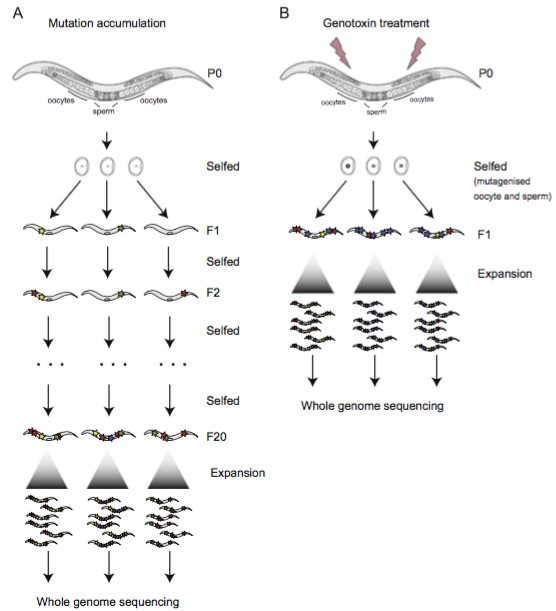
\includegraphics[scale=0.7]{two_exp_types.jpg}}
  \caption{Scheme of two worm experiment types. From Meier et al. 2014 \cite{Meier2}}
  \label{exp_types}
\end{figure}

Panel of cytotoxins consists of substances and exposures employed in cancer treatments: alkylating agents aflatoxin, cisplatin, dimethyl sulfate (DMS), ethyl methanesulfonate (EMS), methyl methanesulfonate (MMS), mechlorethamine (Mech) and hydroxyurea (HU), ionizing gamma-irradiation and X-rays.
List of genetic knock-outs includes genes representing all crucial DNA repair pathways: we consider 6 genes responsible for translesion synthesis, 13 backgrounds associated with single-strand break repair deficiency, 28 conditions associated with double-strand breaks repair deficiency, 6 helicases with different additional properties, 7 DNA damage checkpoint genes and 5 genes related to damage-caused cell death.
Full list of genetic conditions with respective pathways and their effects on genomic stability can be find in the Appendix.


\subsubsection*{Variant calling}

NGS data obtained from the experimental samples with Illumina sequencing at WTSI was further analyzed to extract genomic variants. Variant calling was performed separately for single nucleotide variants, small indels and large structural variants. The results have undergone a thorough filtering procedure to exclude technical errors, sequencing artifacts, caller mistakes and germline variance.

Individual SNVs were obtained using CaVEMan (\cite{caveman}) and separated from SNPs. Filtering for substitutions includes:
\begin{itemize}
\itemsep0em
\item uniqueness of each mutation (reported in only one sample)
\item artifacts removal: maximal coverage at the locus under consideration is 150 reads in control sample
\item no reads reporting variant in control sample
\item at least 20 percent of reads in test sample report variant
\item minimal coverage at the locus under consideration is 15 reads for both test and control samples
\item PCR errors identification: at least 1 read reporting variant in both directions
\item indel caused artifacts removal: no more than one read mapped with an indel across the base
\end{itemize}
After filtering, SNVs for every sample were classified into seven classes including dinucleotide substitutions as a separate class.

Indels (later classified into deletions, insertions and deletion-insertions) were called using Pindel (\cite{pindel}) and filtered according to the following criteria:
\begin{itemize}
\itemsep0em
\item uniqueness of each variant (reported in only one sample)
\item artifacts removal: maximal coverage at the locus under consideration is 150 reads in control sample
\item no reads reporting variant in control sample (up to 1)
\item PCR errors identification: at least 1 read reporting variant in both directions
\item no more than 8 repeat units at site
\item no sample in a panel of 5 control worms has variant in more than one read
\item at least 5 reads reporting variant
\end{itemize}

Structural variants were called using WTSI in-house software BRASS (\cite{NZ}), which extracts breakpoints via assembly from paired-end reads mapping. Filtering for the caller output includes quality control in the form of lower threshold for the number of reads reporting the variant, and repetitive events removal by filtering out all the variants reported at least once in the set of reference samples and deleting the intersecting events of the same type between all the samples.

Structural variants were reported in the form of pairs of breakpoints, which were further classified into the following categories:
\begin{itemize}
\itemsep0em
\item[$\square$] Tandem duplications
\item[$\square$] Deletions
\item[$\square$] Inversions
\item[$\square$] Complex events (more than 2 breakpoints classified as one event)
\item[$\square$] Intrachromosomal translocations
\item[$\square$] Interchromosomal translocations
\item[$\square$] Foldbacks (when one inversion-like breakpoint is present, i.e. polymerase is turning around and reversing the DNA without turning back again)
\end{itemize}

The final distribution of variants among different classes after the filtering procedures is shown in Figure N.

%\begin{figure}[h]
%  \centerline{\includegraphics[scale=0.5]{mut_classes.png}}
%  \caption{Overall distribution of mutations across all samples. Classes from "C$>$A" to "T$>$G" represent substitution classes, "NN$>$NN" - dinucleotide substitutions, "D" - small deletions, "I" - small insertions, "DI" - small deletion-insertions, "TD" - tandem duplications, "DEL" - large deletions, "INV" - invertions, "TRSL" - intrachromosomal translocations.}
%  \label{mut_distr}
%\end{figure}



\subsubsection{Homozygous and heterozygous mutations across generations}







\subsubsection{Extraction of mutational patterns}


\subsubsection*{Assumptions}

\textbf{Overdispersion modeling}. The current data shows signs of significant overdispersion for most of the response classes: residual deviance (i.e. the difference in likelihood for the model under consideration versus saturated) is significantly greater than the residual degree of freedom.



This is probably due to the limitations mentioned earlier: in some cases there was not enough time to see any mutations, which does not allow us to extract the corresponding factor contribution. The presence of overdispersion makes the current estimates of coefficient standard errors biased, which leads to incorrect assessment of coefficients significance and reduced prediction variance (\cite{overdisp}).

In order to account for an excess of zero results, we will turn to Gamma-Poisson model (also known as negative-binomial model), setting a Gamma prior on the coefficients as in \cite{Ivek} and \cite{BNB}, which will help to correctly estimate the actual variance of the result and make better predictions.

\textbf{Model quality assessment}. At the moment we estimate the confidence intervals for coefficients via bootstrapping to confirm stability of the estimates. The prediction error will be calculated by cross-validation procedure.

\textbf{Pattern identification}. We are going to perform unsupervised non-parametric clustering on the initial spectra utilizing hierarchical Dirichlet processes (\cite{Teh}), and try to map clusters to the signatures we extracted in order to confirm the ability to map the calculated effects back to the groups where they were applied.

\subsubsection*{Model}

To assess the individual contributions of every factor, we employed positive Poisson additive model with $r$ responses (reflecting the variant classes), that includes $k$ genetic, mutagenic, gene interaction and gene-mutagen interaction factors, for every response class $j$:

\[Y_{j} \sim Pois(\lambda_{j}), \lambda_{j} \in  \mathbb{R}_{+} , j = 1, ..., r\]

\begin{equation}
E[Y_j] = \lambda_j = X \beta_{j}^{T} = X_{gen} \beta_{j,gen}^T + X_{mut} \beta_{j,mut}^T + X_{int} \beta_{j,int}^T, \beta_j \in (\mathbb{R}_{+} \cup {0})^k
\end{equation}

To extract the model parameters, we further implemented non-negative matrix factorization with generalized Kullback-Leibler divergence minimization:

\[D(A||B) = \sum_{i,j} A_{ij} log(\frac{A_{ij}}{B_{ij}} ) - A_{ij} + B_{ij}\]

This approach is equivalent to maximum likelihood estimation in non-negative Poisson regression model in the case of fixed multiplier $X$: 

\[Y = X \beta, \beta \in M_{k \times r} (\mathbb{R}_{+} \cup {0})\]

\begin{equation}
\begin{split}
\ell(Y|X,\beta) &= \sum_{i,j} \left[Y_{ij}  log⁡(X \beta)_{ij} - (X \beta)_{ij} \right] + C \\
&= - \sum_{i,j} \left[Y_{ij}  log⁡ \left( \frac{Y_{ij}}{(X\beta)_{ij}} \right) - Y_{ij} + (X\beta)_{ij} \right] + \tilde{C} \\ 
&= - D(Y||X\beta) + \tilde{C}
\end{split}
\end{equation}

The update rule we used looks as follows:

\begin{equation}
\beta_{ij} \leftarrow \beta_{ij} \cdot \frac{\sum_s \frac{X_{si} Y_{sj}}{(X\beta)_{sj}}} {\sum_t X_{ti}}
\end{equation}

Coefficient matrix $\beta$ was update on every step till both the change in KL generalized distance \(D(Y||X\beta)\) and average change in the elements of $\beta$ reach the certain threshold. 

The variance and significance of the parameters calculated via NMF were estimated using Poisson maximum likelihood estimation and constrained Wald test (\cite{Wald}).


\subsubsection*{Benchmarking}



\subsubsection*{Method comparison}




%%%%%%%%%%%%%%%%%%%%%%%%%%%%%%%%%%%%%%%%%%%%%%%%%%


\subsection{Patterns of mutation accumulation under genotoxin exposure and DNA repair deficiency}


\subsubsection{DNA repair in \textit{C. elegans} and \textit{H. sapiens}}

\subsubsection*{Differences and similarities}

Signatures extracted for different genetic conditions also mostly coincide with the expected effects based on the function of the genes (\cite{p53}, \cite{Meier1},\cite{DNArepair}, \cite{DNAdamagerepair}). In the examples in the Figure N the following effects are presented: impact of ageing, \textit{brc-1} - BRCA1 ortholog encoding gene which contributes to homologous recombination, \textit{cep-1} - P53-like protein encoding gene which regulated damage-caused cell apoptosis, and \textit{smg-1} - kinase-related protein kinase SMG1 which regulates oxidative stress response.

\subsubsection*{Mutational signatures in mutations per generation}

\textit{rev-1} gene encodes an ortholog of human translesion polymerase REV1 which helps polymerases epsilon and delta to overcome stalled replication fork by inserting cytosins at abasic sites. As shown in Figure N, knocking out this gene does not significantly affect the mutational spectra in mutation accumulation experiment, but remarkably expands the mutational effects of DMS, which normally produces base substitutions and frameshift mutations and deletions.

\textit{xpa-1} encodes an ortholog of the human zinc finger protein XPA involved in nucleotide excision repair, which does not produce mutations when knocked-out alone, but expands the substitution mutational effects of alkylating agents and Gamma-irradiation, as shown in Figure N.





\subsubsection{Genetic interactions}

Apart from quantifying per-generation mutation rates for various knock-outs and effects of mutagen exposure, we have also identified several significant interaction effects, the underlying biology of which needs further investigation.

One example of a significant interaction between genetic backgrounds is the epistatic effect observed between mismatch repair system components \textit{pms-2} and \textit{pole-4}. \textit{pms-2} is a component of mismatch repair complex formed by attachment to \textit{mlh-1}. Both of these genes produce similar remarkable effects spectra when knocked-out, which agrees with the underlying biology (\cite{Denver}).

\textit{pole-4} is a catalytic subunit 4 of the ortholog of human polymerase epsilon, which is assumed to have mostly repair function correcting the errors made by polymerase delta. When knocked out on its own, this gene does not cause significant changes in the samples, but the double mutants with both defective \textit{pms-2} and defective \textit{pole-4} show a 3-fold increase in the overall mutation amount. Deficiencies in human polymerase epsilon and polymerase delta were previously reported as driver genes in hypermutated brain cancers (\cite{Shlien}).





\subsubsection{Mutagen exposures}

Using this approach, we calculated the qualitative effect estimations for all of the factors. Effects for genotoxins used in the study are consistent with their chemical interactions with DNA known from literature (\cite{Helleday}, \cite{DNAdamagerepair}, \cite{Meier1}) and can be found in Figure N.





\subsubsection{Relation to various genomic features}

\subsubsection*{Transcription}

\subsubsection*{Replication directionality}

\subsubsection*{Localisation of mutations}

Microhomology, telomeres, clusters

\subsubsection*{Epigenetic features}

\textbf{Incorporation of additional genetic information}. This includes validation of structural variants (namely, deletions and duplications) by analyzing copy number changes in the sample genomes, GC-content adjustment for correct comparison of substitutions types proportions, and removal of variants coming from low-complexity regions and highly repetitive regions. 

\subsubsection*{Mitochondrial DNA}

%%%%%%%%%%%%%%%%%%%%%%%%%%%%%%%%%%%%%%%

\subsection{Translation of mutational signatures between model organisms and human cancers}

\subsubsection{Mutational patterns of mismatch repair}

\subsubsection{Other DNA repair pathways}

\subsubsection{Differences and similarities in response to mutagen exposure}

Relevance to cancer

DNA repair pathways

Mutagens, cancers related to environmental exposure



%%%%%%%%%%%%%%%%%%%%%%%%%%%%%%%%%%%%%%%

\subsection{Limitations of the analysis}


The current model concept does not account for several limitations coming from the nature of the data:
\begin{itemize}
\itemsep0em
\item Restricted number of mutations - some rearrangement can not be produces in sufficient number (negative selection)
\item Small number of replicates for each experiment (makes it hard to estimate the variance of the results)
\item Negative selection: some rearrangements can not be reproduces in sufficient number (amount of junk DNA is extremely low)
\end{itemize}

To make the model as useful as possible, at the moment we are working on the following aspects:

\subsection{Discussion}




%\newpage{}

%\appendix
%\section*{Appendix. Table of genetic knock-outs and mutagens used in the study with their interactions.}

%\begin{table}[h!]
%\centering
%\begin{adjustbox}{width=1\textwidth}
%\begin{tabular}{1.0*\textwidth}{|c|c|c|c|c|c|c|c|c|c|c|c|}
%\hline 
% & None & Aflatoxin & Cisplatin & DMS & EMS & HU & Mec & MMS & Rad & Xray & Pathway\tabularnewline
%\hline \hline
%N2 & allsubs, D, I, allSVs - INV  &  C$>$A & C$>$A, D & T$>$C, T$>$A, C$>$T, TD & allsubs, D  & C$>$T, C$>$A & D & allsubs – C$>$G, D, TD & allsubs, D & C$>$T, C$>$A, D, TD, INTCHR & \tabularnewline
%\hline 
%agt-1 & TD & & & & C$>$T, T$>$A & T$>$C, T$>$A, C$>$T &  &  &  &  & translesion synthesis	\tabularnewline
%\hline 
%\end{tabular}
%\label{app_table}
%\end{adjustbox}
%\end{table}

\end{document}